\documentclass[a4paper,parskip=half-]{scrartcl}
\usepackage[utf8]{inputenc}
\usepackage[english]{babel}
\usepackage{fancyhdr}
\usepackage{graphicx}
\usepackage{hyperref}
\usepackage{amsmath}
\graphicspath{{c://users//fmeyer//git//ml_ss20/files/graphics/}}
\pagestyle{fancy}
\fancyhf{}
\rhead{
	\small 
		\begin{tabular}[t]{l}
		\textsf{Fabian Meyer, 6816480}\\
		\textsf{Theresa Naß, 7122946}\\
		\end{tabular}}
\lhead{Machine Learning}
\cfoot{	\url{https://github.com/gitfabianmeyer/ml_ss20}}



\begin{document}
	\section{Binary Classification through Logistic Regression}
	In this exercise, we solved a Binary Classification problem using Logistic Regression.
	As the data points were linearly separable, we used a model of form $z = \theta_0 + x_1 *\theta_1 + x_2 * \theta_2$. \\The final model, visualized in Section \ref{plots} is of the form 
	$$x_2 = (\theta_0 + x_1 *\theta_1) (-1/\theta_2). $$
	\subsection{Final Model}
	
	The final model, e.g. the model were every point is classified correctly has the following parameter:
	\begin{align*}
		\alpha &= 0.05\\ 
		\theta_0 &= 7.042258968144114 \\
		\theta_1 &= -1.0005940726111886 \\
		\theta_2 &= 2.9762343453321742\\
	\end{align*}
	
	The next section shows the resulting model, where the black curve is the fitted model. The green the green curve shows the inital model with random, initialized parameter $\theta_j \in [-0.1,0.1]$. We trained the model using the stochastic gradient descent method. 
	
	\subsection{Plots}\label{plots}
	\begin{figure}[!h]
	\centering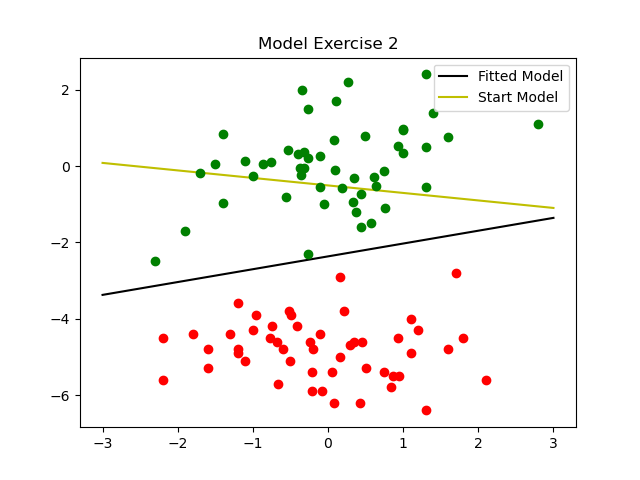
\includegraphics[width=0.6\linewidth]{model_ex2}
	\end{figure}

\end{document}
